\section{Background in Distributed Systems on Cloud}

The previous section introduced the QUIC protocol and all protocols that it’s either trying to improve, or their previous versions. Their differences and motivations were defined and will be used to explain the results of the experiments described further ahead.

In order to understand the experiment's motivations, this section provides an overview of the challenges to build distributed applications on cloud and what they offer to be used in production environments by many large scale companies.

\subsection{Distributed Systems}

Back in the day, the most common way to solve a computing problem was to write a single application that was responsible for performing some kind of task. These applications are called monolithic applications.

Once the application grows to a point it demands scaling, it will demand more replicas of itself to be able to handle more traffic. Though this might not be a problem, since all functionality was incorporated into a single application, in most cases, only a few parts will actually require scaling. Consequently, resulting in a waste of resources.

Distributed systems come into the scene to try solving these problems. It makes use of multiple computing devices spread over a network and have them coordinate efforts to perform some kind of task \cite{distributed_systems_principles}. It allows complex applications to be broken down into manageable chunks, each performing a different kind of functionality.

Its components can be broken down into two categories of clients: ephemeral and persistent.

An ephemeral client creates a single connection to the server, performs some sort of exchange of data, and then closes the connection once it’s finished. A common example is that of a job, a finite task that has to perform a large computation, batch-oriented tasks, or creating a database backup \cite{os_distributed_systems}.

A persistent client, however, also establishes a single connection to the server, but it maintains it open throughout its entire lifetime, making requests when needed. This can be represented by a service that needs to communicate with a database to provide some kind of functionality.

By defining these components and how they work, simulations can be performed to see how they perform on different scenarios. This allows for speculation about their behaviour in a real-world scenario.

\subsection{Cloud}

The term “cloud” was used to refer to platforms for distributed computing as early as 1993 \cite{what_is_cloud}. Cloud computing the delivery of computing services, such as databases and storage, over the Internet. It can be divided into three main categories: \gls{iaas}, \gls{paas}, and \gls{saas}. From here on, the focus will be the \gls{iaas} cloud computing category.

\subsubsection{\gls{iaas} \& Containerization}

\gls{iaas} is a form of cloud computing that has become one of the most common ways to provision on-demand availability of infrastructure services without having to be directly managed by the user \cite{what_is_cloud}.

Users are not required to have their own data centers to be able to serve their applications, they can request resources to use a third party’s computing infrastructure using a pay-as-you-go method. Therefore, they only need to pay for the resources actually used, enabling them to easily scale when needed.

Multi regional servers are also possible. Users are able to request resources in distinct regions to deal with traffic from different countries or due to some contractual requirements. Some providers even have more than one data center per region, capaciting users to build high availability systems that are able to deal with disaster scenarios, for instance the data center experiences a power outage.

As data centers machines processing power and capacity increased over the years, many resources never got to be used by the applications whereas their requirements were much lower. This causes a waste of computing resources that could otherwise be used by users, increasing providers’ revenue. Thus, \glspl{vm} came into existence. 

\gls{vm}s consist of the virtualization of an \gls{os}, allowing one single physical host machine to have more than one virtual machine running at the same time while keeping them isolated from each other \cite{what_is_cloud}. This enables cloud providers to optimize the use of their resources by serving multiple \gls{vm}s while only having to use one physical host machine, consequently serving more than one user per machine.

Nevertheless, \gls{vm}s improve data centers resource efficiency, it can take up a lot of system resources. Each \gls{vm} requires a copy of an \gls{os} and a virtual copy of all the hardware that the \gls{os} needs to run, adding up to a lot of memory and \gls{cpu}. This is still more efficient than running separate physical host machines, but can be a deal-breaker for applications.

To improve application development, deployment and flexibility, containers were created. Instead of virtualizing the entire host machine, containers use linux namespaces to run on isolated environments while sharing the underlying \gls{os} (Figure \ref{figure:vm_vs_container}), resulting in less requirements since they only need to package the actual application and all files necessary to run. In addition, their lightweight characteristic allows faster startup time, while \gls{vm}s may take minutes to be provisioned, most containers are ready in a few milliseconds.

\begin{figure}[ht]
    \centering
    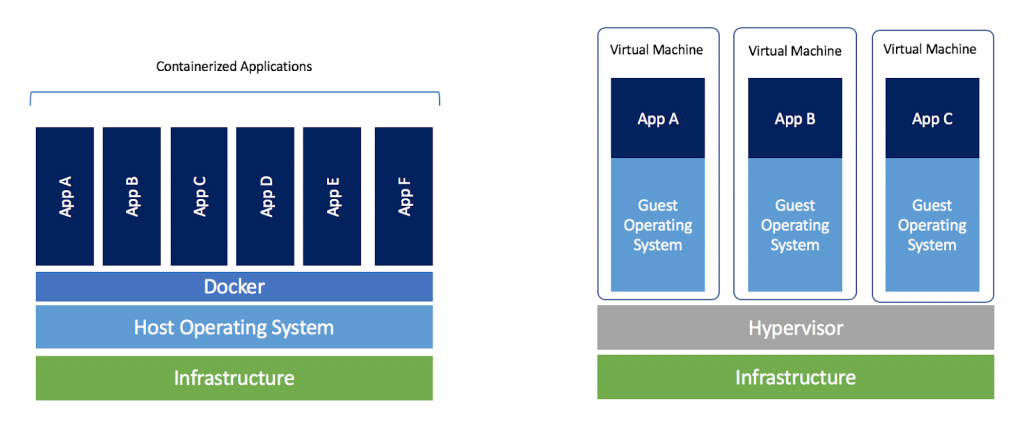
\includegraphics[width=\linewidth]{figures/Blog.-Are-containers-..VM-Image-1-1024x435.png}
    \caption{Containers versus Virtual Machines}
    {Source: \cite{are_containers_replacing_virtual_machines}}
    \label{figure:vm_vs_container}
\end{figure}

Developers usually write code locally possibly using their laptop, and then this code will be deployed on the server. Any differences between these two environments, laptop and server, can cause unexpected bugs. Containers solve the problem of environment inconsistency. Developers can work on a local environment that contains all of the dependencies of any environment whether it’s development, testing, or production.

\subsubsection{Kubernetes}

Dealing with distributed systems over the cloud have given companies the power to build complex and intelligent solutions that are able to solve really hard problems that otherwise would require a lot of investment and time. However, managing such systems comes with its own challenges.

Due to containers being lightweight and ephemeral, running them in a production environment can become overwhelming. A containerized application might need to operate hundreds to thousands of containers. A container orchestrator is the automation of operational effort required to run such containerized applications.

According to the \gls{cncf}, \gls{k8s} is an open source container orchestration engine for automating deployment, scaling, and management of containerized applications \cite{kubernetes}. Additionally, it’s considered the most widely used container orchestration platform by \gls{cncf}’s \gls{k8s} Project Journey Report from 2019 \cite{cncf_k8s_report}.

The fundamental premise behind \gls{k8s} is that it enforced desired state management. Consequently, a \gls{k8s} cluster is fed with specific configuration files, called manifests, and it's up to the cluster to provide the necessary infrastructure to be able to meet the desired state.

\gls{k8s}’ smallest and most basic deployable object is called pod. It consists of a wrapper around containers that has computing resources. One or more containers can be inside a single pod, consequently sharing the pod’s resources with each other.

In the context of containers, a pod is a set of Linux namespaces and the same things that are used to isolate a container. Therefore, in the context of \gls{k8s}, it’s common to refer to pods when talking about scaling and deployment.

Each cloud provider often provides a managed way of running \gls{k8s}, they take care of the control plane, component responsible for managing the worker nodes and the pods, management while enabling users to actually use the cluster to their needs. For instance, \gls{aws} offers the \gls{eks}.

Some cloud providers allow applications to be deployed in different regions. In the case of \gls{aws}, it even allows you to choose a data center within a region, defined as \gls{az}. Hence, there can be multiple \gls{az}s within a single region.

Within the \gls{k8s} it’s possible to have pods deployed to different regions or \gls{az}s based on their affinity and tolerations by tainting a node with a label. This allows the user to have full control over where each application is going to run.

\subsection{Summary}

This section finished all required aspects of managing distributed systems on cloud. Therefore, their challenges and benefits should be clear, as well as their importance to the computing world.

The next section will bring details on how the implemented Benchmark Service will perform experiments. They are going to put previously described protocols to the test in a cloud environment. Consequently, being able to assess their results.
